\documentclass{ximera}

\newcommand{\RR}{\mathbb R}
\renewcommand{\d}{\,d}
\newcommand{\dd}[2][]{\frac{d #1}{d #2}}
\renewcommand{\l}{\ell}
\newcommand{\ddx}{\frac{d}{dx}}
\newcommand{\dfn}{\textbf}
\newcommand{\eval}[1]{\bigg[ #1 \bigg]}


\outcome{Use ``shortcut'' rules to find and use derivatives.}
\outcome{Use the definition of the derivative to develop a shortcut
  rule to find the derivative of the natural exponential function.}

\title[Dig-In:]{The derivative of the natural exponential function}

\begin{document}
\begin{abstract}
  We derive the derivative of the natural exponential function.
\end{abstract}
\maketitle

We don't know anything about derivatives that allows us to compute the
derivatives of exponential functions without getting our hands
dirty. Let's do a little work with the definition of the derivative:
\begin{explanation}
\begin{align*}
\ddx a^x &=\lim_{h\to 0} \frac{a^{x+h}-a^x}{h} \\
&=\lim_{h\to 0} \frac{a^xa^{h}-a^x}{h} \\
&=\lim_{h\to 0} a^x\frac{\answer[given]{a^{h}-1}}{h} \\
&=a^x\lim_{h\to 0} \frac{a^{h}-1}{h} \\
&=a^x \cdot \underbrace{\text{(constant)}}_{\lim_{h\to 0} \frac{a^{h}-1}{h}}
\end{align*}
\end{explanation}
There are two interesting things to note here: We are left with a
limit that involves $h$ but not $x$, which means that whatever $
\lim_{h\to 0} (a^h-1)/h$ is, we know that it is a number, or in other words, a
constant. This means that $a^x$ has a remarkable property:
\begin{quote}
  \textbf{The derivative of an exponential function is a constant
    times itself.}
\end{quote}
Unfortunately it is beyond the scope of this text to compute the limit
\[
\lim_{h\to 0} \frac{a^h-1}{h}.
\]
However, we can look at some examples. Consider $(2^h-1)/h$ and $(3^h-1)/h$:

\begin{image}
  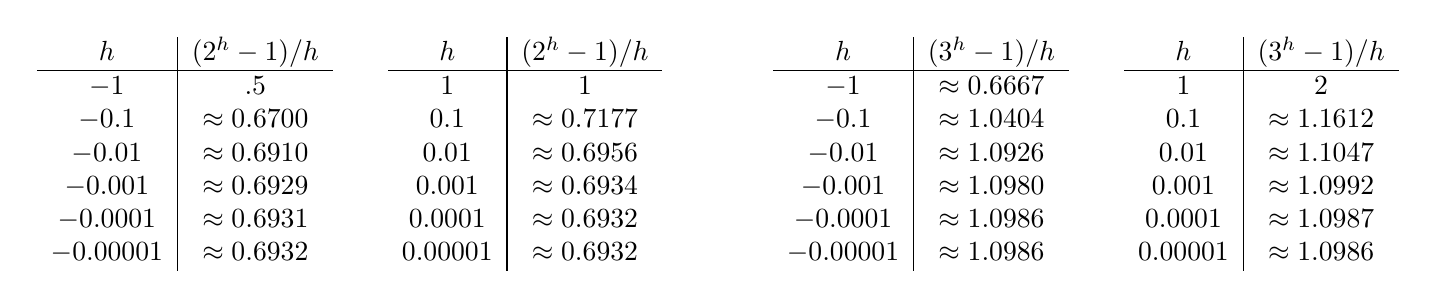
\begin{tikzpicture}
    \node at (0,0) {$\begin{array}{c|c}
 h &     (2^h-1)/h\\ \hline
 -1 & .5  \\
-0.1 &  \approx0.6700 \\
-0.01 & \approx0.6910 \\
-0.001 & \approx0.6929 \\
-0.0001 & \approx0.6931 \\
-0.00001 & \approx0.6932 \\
\end{array}
\qquad
\begin{array}{c|c}
 h &     (2^h-1)/h\\ \hline
 1 & 1  \\
 0.1 &  \approx0.7177 \\
 0.01 & \approx0.6956 \\
 0.001 & \approx0.6934 \\
 0.0001 & \approx0.6932 \\
 0.00001 & \approx0.6932 \\
\end{array}
\qquad\qquad
\begin{array}{c|c}
 h &     (3^h-1)/h\\ \hline
-1 & \approx 0.6667  \\
-0.1 &  \approx1.0404  \\
-0.01 & \approx1.0926 \\
-0.001 & \approx1.0980 \\
-0.0001 & \approx1.0986 \\
-0.00001 & \approx1.0986 \\
\end{array}
\qquad
\begin{array}{c|c}
 h &     (3^h-1)/h\\ \hline
 1 & 2  \\
 0.1 &  \approx1.1612 \\
 0.01 & \approx1.1047 \\
 0.001 & \approx1.0992 \\
 0.0001 & \approx1.0987 \\
 0.00001 & \approx1.0986 \\
 \end{array}$};
\end{tikzpicture}
\end{image}



While these tables don't prove that we have a pattern, it turns out that
\[
\lim_{h\to 0}\frac{2^h-1}{h} \approx .7 \qquad\text{and}\qquad \lim_{h\to 0} \frac{3^h-1}{h} \approx 1.1.
\]
Moreover, if you do more examples, choosing other values for the 
base $a$, you will find that the limit varies
directly with the value of $a$: bigger $a$, bigger limit; smaller $a$,
smaller limit. As we can already see, some of these limits will be
less than $1$ and some larger than $1$. Somewhere between $a=2$ and $a=3$
the limit will be exactly $1$. This happens when 
\[
a = e = 2.718281828459045\dots.
\]
We will define the number $e$ by this property, see the next
definition:
\begin{definition}\index{e@$e$}
  The number denoted by $e$, called \dfn{Euler's number}, is defined
  to be the number satisfying the following relation
  \[
  \lim_{h\to 0} \frac{e^h-1}{h} = 1.
  \]
\end{definition}
Using this definition, we see that the function $e^x$ has the following truly remarkable property.

\begin{theorem}[The derivative of the natural exponential function]\index{ex@$e^x$}\index{derivative!of ex@of $e^x$}
The derivative of the natural exponential function is the natural exponential function itself.  In other words,
\[
\ddx e^x = e^x.
\]
\begin{explanation}  
From the limit definition of the derivative, write
\begin{align*}
\ddx e^x&=\lim_{h\to 0} \frac{e^{x+h}-e^x}{h} \\
&=\lim_{h\to 0} \frac{e^xe^{h}-e^x}{h} \\
&=\lim_{h\to 0} \answer[given]{e^x}\frac{e^{h}-1}{h} \\
&=e^x\lim_{h\to 0} \frac{e^{h}-1}{h} \\
&=e^x.
\end{align*}
\end{explanation}
\end{theorem}


Hence $e^x$ is its own derivative. In other words, the slope of the
plot of $e^x$ is the same as its height, or the same as its second
coordinate.  Said another way, the function $f(x)=e^x$ goes through the point $(a,e^a)$
and has slope $e^a$ at that point, no matter what $a$ is. 

\begin{question}
  What is the slope of the tangent line to the function $f(x) = e^x$ at $x = 5$?
  \begin{prompt}
    The slope is $\answer[given]{e^5}$.
  \end{prompt}
\end{question}



\begin{example}
Compute:
\[
\ddx\left(8\sqrt{x} + 7e^x \right)
\]
\begin{explanation}
Write with me:
\begin{align*}
\ddx\left(8\sqrt{x} + 7e^x \right) &= 8\ddx x^{1/2} + 7\ddx e^x\\
&= 4x^{-1/2} + 7 \answer[given]{e^x}.
\end{align*}
\end{explanation}
\end{example}


\end{document}
